\section{Experiments}\label{sec:exp}

\subsection{Heuristics}
We design many heuristics for both A* and RBFS. Here we show an admissible one and two non-admissible ones for demonstrating. Other heuristics will be discussed in section \ref{sec:dis}.

An admissible heuristic is designed by simulating the game of tower. For the second and third peg, disks on there should be moved to the first peg. An admissible esitimation of steps is the amount of disks in these pegs. If a disk on the bottom of peg 1 is not the right one, it should be moved out first and then move to its ideal position, which takes at least $2k$ steps, where k is the number of disks on top of it. We show the heuristic below:
\[
h1(s) = I(s(1,0)==goal(1,0))\cdot 2 \cdot num(s(1)) + num(s(2)) + num(s(3))
\]
Here $I(\cdot)$ is indication function, and $num(\cdot)$ is the function for counting disks. A non-trivial non-admissible heuristic is designed in a similar way but taking ordering into account:
\[
h2(s) = (\sum_i |s(1,i)-i| ) + numberDisks(s(2)) + numberDisks(s(3))
\]
Here s(i,j) is the $jth$ disks in peg $i$. The intuition is that for a disk $k$ in peg $1$, it has to take $|k-i|$ steps to get to the $kth$ place by moving away or filling out disks on peg $0$, where $i$ is its current location on the peg. For example, if the $9th$ disk is on the bottom, it has to take $9-0$ steps to get to the top. For disks on peg $2$ and peg $3$, they have to be moved from the current location to peg $1$ in at least $1$ step, which are the same as admissible
heuristic. However this is not an admissible heuristic because there are multiple counts for disks on peg $0$. 

For a fast non-admissible heuristic, we simplily enlarge the former heuristic by a factor of $2$. we will see this relaxion makes the increasing of computation and expanded nodes becomes linear in problem size ranging from $4-10$.
\[
h3(s) = 2 \cdot [(\sum_i |s(1,i)-i| ) + numberDisks(s(2)) + numberDisks(s(3))]
\]
\subsection{Results}

\begin{figure}[!t]
\centering
\begin{tabular}{cc}
\subfloat[A* nodes: all 140 experiments]{\includegraphics[scale=0.32]{img/tnode_Astar.pdf}} 
   & \subfloat[RBFS nodes: all 140 experiments]{\includegraphics[scale=0.32]{./img/tnode_RBFS.pdf}}\\
\subfloat[A* average searched nodes]{\includegraphics[scale=0.32]{./img/anode_Astar.pdf}} 
   & \subfloat[RBFS average searched nodes]{\includegraphics[scale=0.32]{./img/anode_RBFS.pdf}}\\
%\subfloat[E]{\includegraphics[width=2cm]{logo}} 
%   & \subfloat[F]{\includegraphics[width=3cm]{logo}}\\
\end{tabular}
\caption{Plots for the number of nodes searched against the problem size for each algorithm and heuristic. For the first 2 figures, number of disks within 4-10, every 20 examples have the same problem size. We show average expanded nodes against number of disks for a clear demonstration. As the problem size becomes larger, the number of searched nodes grow up exponentially.}
\label{fig:nodes}
\end{figure}

\begin{figure}[!t]
\centering
\begin{tabular}{cc}
\subfloat[A*: average cpu time (s) on heuristics]{\includegraphics[scale=0.32]{./img/AHcpu-aver.pdf}} 
   & \subfloat[RBFS: average cpu time (s) on heuristics]{\includegraphics[scale=0.32]{./img/RHcpu-aver.pdf}}\\
\subfloat[A*: average cpu time (s) on whole problem]{\includegraphics[scale=0.32]{./img/ATcpu-aver.pdf}} 
   & \subfloat[RBFS: average cpu time (s) on whole problem]{\includegraphics[scale=0.32]{./img/RTcpu-aver.pdf}}\\
%\subfloat[E]{\includegraphics[width=2cm]{logo}} 
%   & \subfloat[F]{\includegraphics[width=3cm]{logo}}\\
\end{tabular}
\caption{Plots for the average cpu time against the problem size over 20 examples for each algorithm and heuristic.}
\label{fig:cputime}
\end{figure}

\begin{figure}[!t]
\centering
\begin{tabular}{cc}
\subfloat[Nodes against disks for admissible heurisitic]{\includegraphics[scale=0.32]{./img/node_Astar_RBFS_H_ad.pdf}} 
   & \subfloat[Nodes against disks for non-admissible heurisitic]{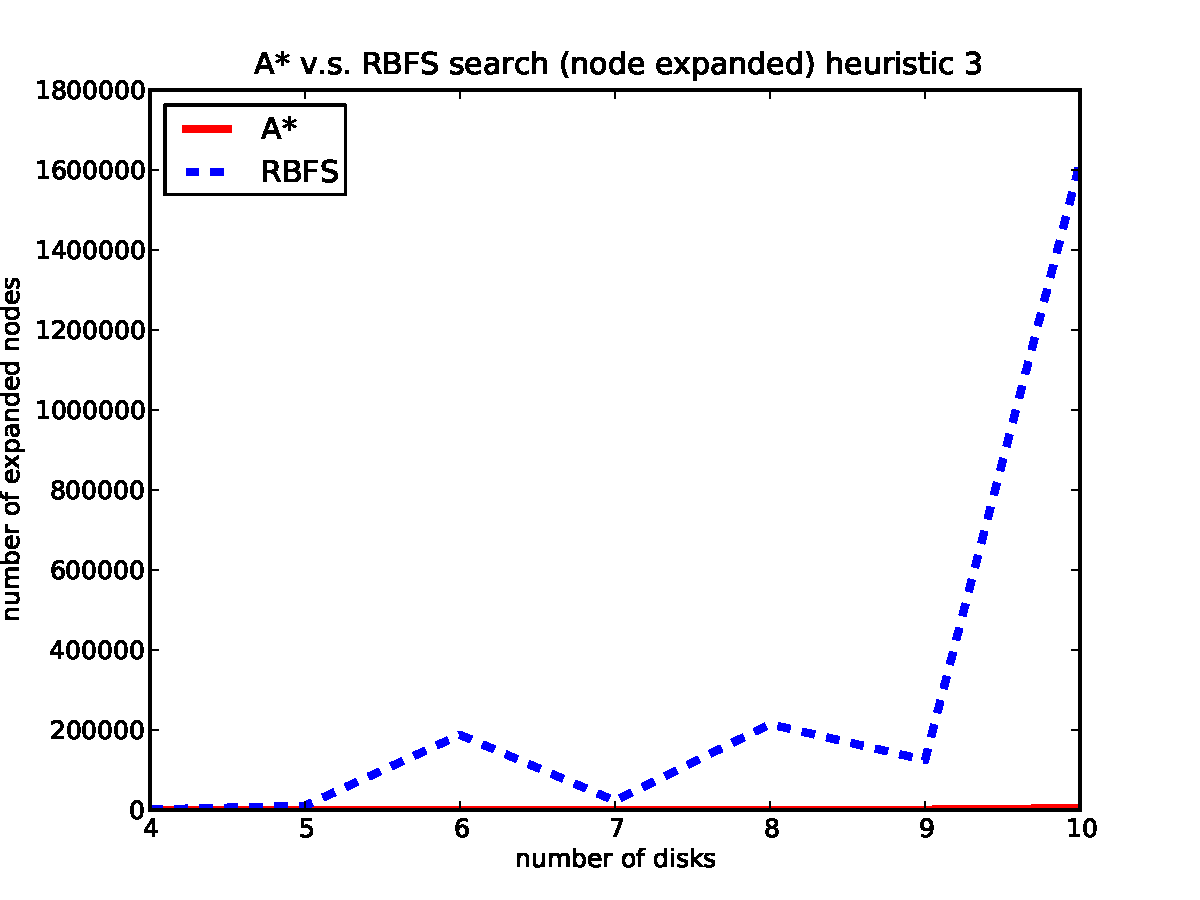
\includegraphics[scale=0.32]{./img/node_Astar_RBFS_H_nad.pdf}}\\
%\subfloat[cpu time against disks for heurisitic 1]{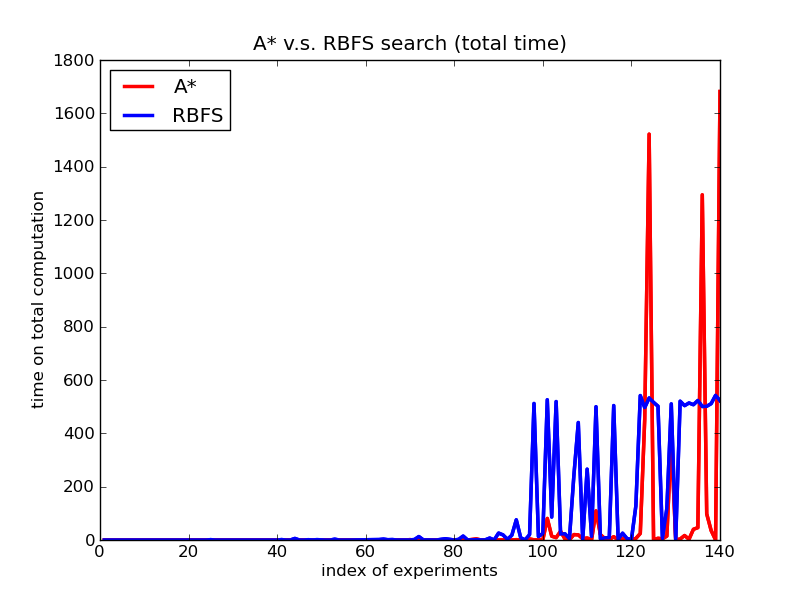
\includegraphics[scale=0.32]{../results/Astar_RBFS_H1_cpu.png}} 
   %& \subfloat[cpu time against disks for heurisitic 2]{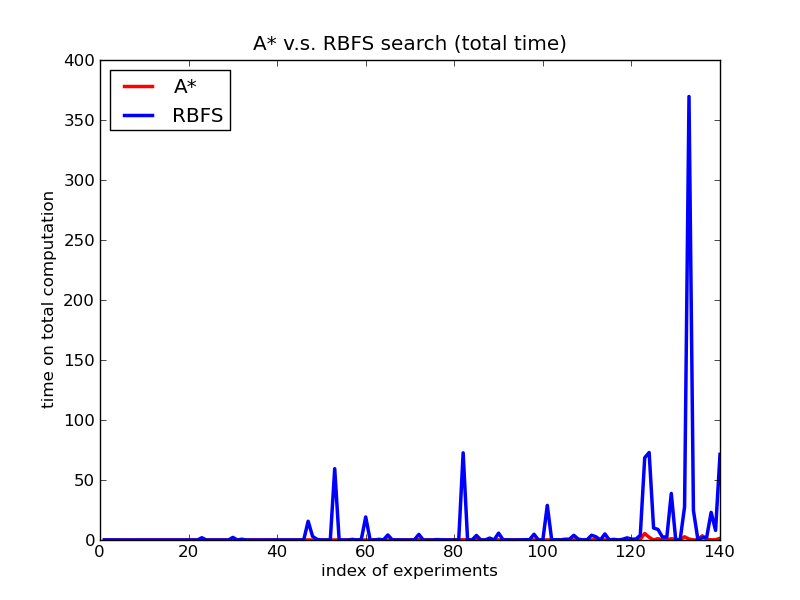
\includegraphics[scale=0.32]{../results/Astar_RBFS_H2_cpu.png}}\\
\end{tabular}
\caption{Performance comparisons between A* and RBFS}
\label{fig:astar-rbfs}
\end{figure}


We tested the three heuristics on all 140 examples for the problem size ranging from $4-10$, each size has $20$ examples. We couldn't finish the admissible heuristic on whole data. For large size like $9$ or $10$, a few examples take more than one hour. For RBFS, the expanded nodes grow up rapidly and failed to maximum limitation. We show $4-9$ for admissible heuristic (heuristic 1) and whole data for non-admissible heuristics (heuristic 2 and 3). 

The first and second experiment are comparisons of expanded nodes and cpu time between different heurisitics, which are shown in figure \ref{fig:nodes} and figure \ref{fig:cputime} respectively. We can see that both nodes and cpu time grow up expenentially. However, a well designed heuristic function can control the increasing in a certain range. It may not lead to optimal solution but efficient for real-time problem. 

We also compared A* and RBFS (figure \ref{fig:astar-rbfs}), we found the trendencies expanded nodes and cpu time are similar, so we only show the nodes comparison. A* outperforms RBFS in terms of cpu time and searched nodes. From figure \ref{fig:cputime}, we can see RBFS spends $1/3$ of whole cpu time on heuristic computation while A* takes less than $1$ second. This is because RBFS expanding more nodes than A*, every node has to compute a heuristic value.

The average solution lengths are shown in table \ref{tab:solen}. Because some experiments are failed in RBFS for reaching the maximum limitation of expanded nodes, the average lengths of admissible RBFS are a little bit smaller without these examples. All values are not far away. It suggests non-admissible heuristics are also reasonable choices for large scale problems.

\begin{table}[!h]
    \centering
    \scalebox{0.9}{
	    \begin{tabular}{|l|c|c|c|c|c|c|c|}
		\hline
		Disks: & 4 & 5 & 6 & 7 & 8 & 9 & 10\\ \hline
		A*/admissible & 8.8 & 11.6 & 13.95 & 16.5 & 18.6 & n/a & n/a\\ \hline
		%A*/admissible H7 & 8.95 & 11.6 & 13.95 & 16.75 & 19.2 & 22.4 & 24.77\\ \hline
		RBFS/admissible & 8.8 & 11.6 & 13.95 & 16.35 & 17.11 & n/a & n/a\\ \hline
		A*/nonadmissible 1 & 8.85 & 11.85 & 14.6 & 17.5 & 20.2 & 24.1 & 27.6\\ \hline
		RBFS/nonadmissible 1 & 8.85 & 11.85 & 15.25 & 19 & 22.21 & 26.81 & 32.25 \\ \hline
		A*/nonadmissible 2 & 9.25 & 12.95 & 16.5 & 20.05 & 23.8 & 27.4 & 34.05\\ \hline
		RBFS/nonadmissible 2 & 11.25 & 17.85 & 24.35 & 32.75 & 40.35 & 50.7 & 64.55\\ \hline
	    \end{tabular}
    }
    \caption{Average solution length per algorithm, heuristic and disk size. n/a means unable to compute within 10 minutes for all problems. Note some experiments failed for reaching the maximum limitation of expanded nodes have been taken out.}\label{tab:solen}
\end{table}


